\documentclass{article}
\usepackage[utf8]{inputenc}
\usepackage[margin=1in]{geometry}

\usepackage{algorithm}
\usepackage[noend]{algpseudocode}
\usepackage{enumitem}

\usepackage{tikz}
\usetikzlibrary{calc,shapes.multipart,chains,arrows,positioning}
\tikzstyle{vertex}=[draw,fill=myseagreen,circle,minimum size=24pt,inner sep=0pt]
\definecolor{myseagreen}{RGB}{240,240,240}

\title{Heavy Light Decomposition}
\author{Daniel Wisdom}
\date{15 March 2019}

\begin{document}

\maketitle



In trees the maximum distance from a node to the root is N.  In some cases where we only need to consider one path of a tree, we can speed this up by compressing nodes into chains.  Heavy-Light decomposition is a method for compressing long paths of nodes in one chain.  We can then travel up the tree from chain to chain, skipping many compressed nodes.

For a node $v$ with many children, we pick the edge to the largest subtree to be the heavy edge.  All the other subtrees are light edges.  If there is tie we can break it arbitrarily.  All non-leaf nodes therefore have exactly one heavy subtree.  Heavy edges form chains that begin at some node and continue to a leaf node.  Every node is part of exactly one chain.

In a subtree of size $N$, a light subtree has less than $N/2$ nodes, or else it would have been the heavy subtree.  This means that, to traverse the tree from the root to any leaf, we only cross $\log N$ light edges.  We also only traverse $\log N$ chains.

Depending on the problem, we usually keep some data/data structure at each chain.  These are often binary indexed trees or segment trees.

\begin{center}
    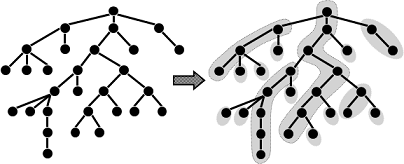
\includegraphics{Heavy-LightDecomposition1.png}
    
    www.csie.ntnu.edu.tw/~u91029/Heavy-LightDecomposition1.png
\end{center}

\section{Example Problem}

Farmer John has a lot of fields of grass connected by bidirectional pathways such that there is exactly one path between any two fields.  Each field has some amount of grass available for eating.  There will be updates mixed with queries.  Updates will set the amount of grass in a specified field.  Queries will ask how much grass is on the path from a specified field to field 0, including both endpoints.

\section{Finding the Decomposition}

We first do a DFS over the tree to find, for each node, its depth and subtree size.  At this point we are ready to construct our data structures for each chain.

We could initialize a segment tree for every chain and set of a system of references to do that, but there is an easier way.  We can create one large segment tree and arrange the base nodes such that every chain is a contiguous sequence of base nodes.  We can do this by recursively traversing the tree, where we first recur on $u$'s heavy child, then place $u$ in the segment tree base, and then recur on all $u$'s light children.  While setting up the chains it is usually helpful to store which chain a node belongs to, and the parent node of each chain.

This only requires running a DFS and building a segment tree, so the runtime is $O(N \log N)$.

\section{Queries and Updates}

If we root the tree and the heavy-light decomposition at field 0, then the queries ask for the sum of nodes from node $v$ to the root.  That just requires walking up that tree using chains.  

We will build  a sum segment tree for each chain.  To walk up the tree starting from node $v$, we will take the range sum of the segment tree from $v$ to the top of $v$'s chain.  We then find the parent of the top of the chain.  This crosses a light edge and brings us to the next chain.  From there we repeat finding the range sum and continue up the tree to the root.  We traverse a maximum of $\log N$ chains, each requiring an $O(\log N)$ range query, so the overall query runtime is $O(\log^2 N)$

To update the grass at a node, we just do a regular segment tree update with the new value.

\section{A Harder Example}

This is the same as the previous example, but each query asks for the largest field on the path between two nodes $a$ and $b$.

We can easily switch out our segment sum trees for segment max trees. That leaves how to deal with queries that do not pass through the root.

If we follow the tree up from any two nodes, their paths will eventually meet at their lowest common ancestor.  We can see the path from $a$ to $b$ as the concatenation of two paths, one from $a$ to the LCA and one from the LCA to $b$.

\begin{figure}[h]
\center
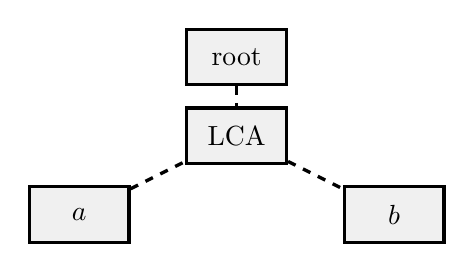
\begin{tikzpicture}[very thick,level/.style={sibling distance=70mm/#1}]
\tikzstyle{vertex}=[draw,fill=myseagreen,rectangle,minimum width=36pt,minimum height=20pt,inner sep=0pt]
\draw (2, 2) node [vertex] (n1) {root};
\draw (0, 0) node [vertex] (n3) {$a$};
\draw (4, 0) node [vertex] (n4) {$b$};
\draw (2, 1) node [vertex] (n2) {LCA};
\draw[dashed] (n1) -- (n2);
\draw[dashed] (n3) -- (n2);
\draw[dashed] (n2) -- (n4);
\end{tikzpicture}
\caption{LCA of two nodes}
\end{figure}

We will use a similar approach as past lectures to find the LCA.  We will move $a$ up the tree as we move $b$ up the tree.  When these two pointers collide, we have found the LCA.  Specifically, we will find the deeper of $a$ and $b$ and advance that one.  We will bring it to the top of its chain and the cross the light edge, putting it on a different chain.  If $a$ and $b$ are now on the same chain, we are done.  Otherwise we repeat moving up the lower pointer.

Once $a$ and $b$ are on the same chain then the higher pointer of $a$ and $b$ is the LCA.  While we move $a$ and $b$ up the tree we can keep the maximum of the chains they pass over, which will almost answer the query.  The final step is to take the range maximum from $a$ to $b$ on the last chain.  This allows us to implicitly find the LCA as we query for the maximum field along the path.

\section{Problems}

\subsection{USACO December 2011, Gold}

Problem 3: Grass Planting [Travis Hance, 2011]

Farmer John has N barren pastures $(2 \leq N \leq 100,000)$ connected by N-1 
bidirectional roads, such that there is exactly one path between any two 
pastures.  Bessie, a cow who loves her grazing time, often complains about 
how there is no grass on the roads between pastures.  Farmer John loves 
Bessie very much, and today he is finally going to plant grass on the
roads.  He will do so using a procedure consisting of M steps $(1 \leq M \leq
100,000)$.

At each step one of two things will happen:

- FJ will choose two pastures, and plant a patch of grass along each road in
between the two pastures, or,

- Bessie will ask about how many patches of grass on a particular road, and 
Farmer John must answer her question.

Farmer John is a very poor counter -- help him answer Bessie's questions!

\subsection{SPOJ: Query on a tree again!}
You are given a tree (an acyclic undirected connected graph) with N nodes. The tree nodes are numbered from 1 to N. In the start, the color of any node in the tree is white.

We will ask you to perform some instructions of the following form:
\newline
0 i : change the color of the i-th node (from white to black, or from black to white);
\newline
1 v : ask for the id of the first black node on the path from node 1 to node v. if it doesn't exist, you may return -1 as its result.


\subsection{SPOJ: Query on a tree 6}

You are given a tree (an acyclic undirected connected graph) with n nodes. The tree nodes are numbered from 1 to n. Each node has a color, white or black. All the nodes are black initially. We will ask you to perform some instructions of the following form:
\newline
0 u: ask for how many nodes are connected to u, two nodes are connected if all the node on the path from u to v (inclusive u and v) have the same color.
\newline
1 u: toggle the color of u (that is, from black to white, or from white to black).

\end{document}
